\setcounter{chapter}{1}
\chapter{Engenharia de requisitos}\label{cap:cap2}

\begin{flushright}
	\textit{
		Um ladrão rouba um tesouro, mas não furta a inteligência. \\
		Uma crise destrói um herança, mas não uma profissão. \\ Não importa se você não tem dinheiro, você é uma pessoa rica, \\ pois possui o maior de todos os capitais: a sua inteligência. \\ Invista nela. \textbf{Estude}!.
	} \\
	
	\textbf{Augusto Cury}
\end{flushright}

Os problemas que os engenheiros de software têm para solucionar são, muitas vezes, imensamente complexos. Compreender a natureza dos problemas pode ser muito difícil, especialmente se o sistema for novo sendo que, um dos pontos que mais dificultam é o conflito entre a visão ampla e o foco, ou seja, muitas vezes o cliente não consegue enxergar as minucias do problema mas somente ele de forma geral. Assim, os engenheiros de software necessitam de meios que os auxiliem na descoberta destas minucias que, juntas, constroem a identidade do software. Portanto, para auxiliar os engenheiros nesta difícil tarefa, foi criada a Engenharia de requisitos. 

\section{Engenharia de Requisitos}

Para que possamos compreender o que é Engenharia de requisitos, devemos entender primeiramente o que é um requisito. 

Um requisito de software, de forma geral, são as  descrições das funções e das restrições de um sistema. Entende-se por função algo que o sistema deve fazer, e por restrição o contrário, o que o sistema não deve executar. Já o processo de descobrir, analisar, documentar e verificar essas funções e restrições é chamado de \textbf{engenharia de requisitos} \cite{sommerville2003engenharia}.

Contudo, para \cite{sommerville2003engenharia}, o termo requisito é usado de forma errada pela industria. Assim, o autor separa a ideia de requisitos em dois grandes  grupos, os quais são:

\begin{enumerate}
	\item \textbf{Requisitos do usuário} são declarações, em linguagem natural e também em diagramas, sobre as funções que o sistema deve fornecer e as restrições sob as quais deve operar.
	\item \textbf{Requisitos de sistema} estabelecem detalhadamente as funções e as restrições de sistema. O documento de requisitos de sistema, algumas vezes chamado de especificação funcional, deve ser preciso. Ele pode servir como um contrato entre o comprador do sistema e o desenvolvedor do software.
\end{enumerate}

Diferentes níveis de especificação de sistema são úteis porque comunicam informações sobre o sistema para diferentes tipos de leitores. A Figura \ref{fig:req-u-s} ilustra a distinção entre os requisitos de usuários e os de sistemas. Ela mostra como um requisito de usuário pode ser expandido em diversos requisitos de sistema.

\begin{figure}[H]
	\centering
	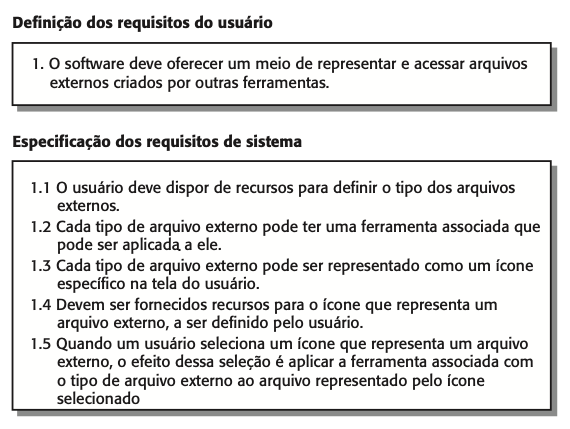
\includegraphics[scale=0.6]{imagens/req-u-s.png}
	\caption{Requisitos do usuário e do sistema. \cite{sommerville2003engenharia}}
	\label{fig:req-u-s}
\end{figure}

\section{Requisitos funcionais e não funcionais}

Os requisitos de sistema de software são, frequentemente, classificados como funcionais ou não funcionais:

\begin{enumerate}
	\item \textbf{Requisitos funcionais:} São declarações de funções que o sistema deve fornecer, como o sistema deve reagir a entradas específicas e como deve se comportar em determinadas situações. Em alguns casos, os requisitos funcionais podem também explicitamente declarar o que o sistema não deve fazer.
	\item \textbf{Requisitos não funcionais:} São restrições sobre os serviços ou as funções oferecidos pelo sistema. Entre eles destacam-se restrições de tempo, restrições sobre o processo de desenvolvimento, padrões, entre outros.
\end{enumerate}

Porém, \citeonline{sommerville2003engenharia} esclarece que, na realidade, a distinção entre esses diferentes tipos de requisitos não é tão clara como sugerem essas definições simples. Um requisito de usuário relacionado à proteção, digamos, parece ser um requisito não funcional. Contudo, quando desenvolvido com mais detalhes, pode levar a outros requisitos que são claramente funcionais, como a necessidade de incluir recursos de autorização de usuários no sistema. Portanto, embora seja útil classificar os requisitos dessa maneira quando os discutimos, devemos lembrar que essa é, na verdade, uma distinção artificial. 

\subsection{Requisitos funcionais}

Segundo \citeonline{nardelliapostila}, requisitos funcionais são conhecidos como a descrição das diversas funções que usuários querem ou precisam que o software faça. Eles definem a funcionalidade desejada do software. O termo função é usado no sentido genérico de operação que pode ser realizada pelo software, seja através de comandos dos usuários ou seja pela ocorrência de eventos internos ou externos ao software.

A especificação de um requisito funcional deve determinar o que se espera que o software faça, sem a preocupação de como ele faz. Por exemplo: 

\textbf{[RF01]} - O software deve permitir que o atendente efetue o cadastro de clientes.

\textbf{[RF02]} - O software deve permitir que o caixa efetue o registro de itens vendidos.

\textbf{[RF03]} - O software deve permitir que o administrador gere um relatório de vendas por mês.

\textbf{Dica:}
Uma boa prática para definição de requisitos funcionais: O software deve permitir que alguém ou alguma coisa realize algo no sistema.

Portanto, baseando-se nas ideias de \citeonline{sommerville2016software}, a princípio, a especificação dos requisitos funcionais de um sistema deve ser \textbf{completa} e \textbf{consistente}. Completude significa que todos os serviços requeridos pelo usuário devem ser definidos. Consistência significa que os requisitos não devem ter definições contraditórias. Lembrando também que o \textbf{documento de requisito não é estático}. Os problemas somente emergem depois de uma análise mais profunda. À medida que os problemas são descobertos durante as revisões ou em fases posteriores do ciclo de vida, os problemas no documento de requisitos devem ser corrigidos \cite{sommerville2003engenharia}.

\subsection{Requisitos não funcionais}

Os requisitos não funcionais, como o nome sugere, são requisitos que não estão diretamente relacionados com os serviços específicos oferecidos pelo sistema a seus usuários. Eles podem estar relacionados às propriedades emergentes do sistema, como confiabilidade, tempo de resposta e ocupação de área \cite{sommerville2016software}. 

Da mesma maneira que os requisitos funcionais podem ser classificados, os requisitos não funcionais também podem de acordo com a sua especificidade: 

\begin{enumerate}
	\item \textbf{Requisitos de produto.} Esses requisitos especificam ou restringem o comportamento do software.
	\item \textbf{Requisitos organizacionais.} Esses são os requisitos gerais de sistemas derivados das políticas e procedimentos da organização do cliente e do desenvolvedor.
	\item \textbf{ Requisitos externos.} Esse tipo abrange todos os requisitos que derivam de fatores externos ao sistema e seu pro- cesso de desenvolvimento.
\end{enumerate}

\begin{figure}[H]
	\centering
	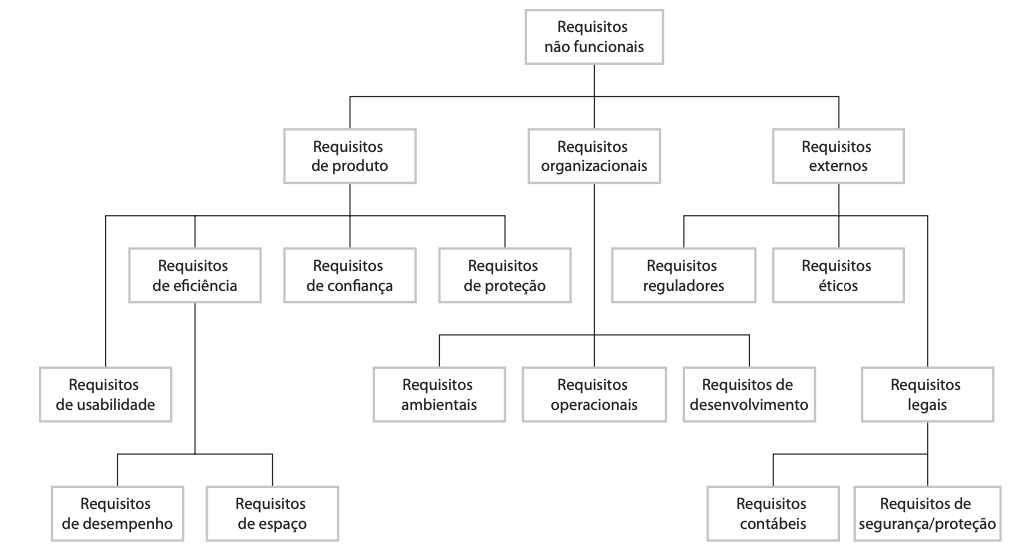
\includegraphics[scale=0.4]{imagens/req-n-funcionais.png}
	\caption{Tipos de requisitos não funcionais \cite{sommerville2016software}}
	\label{fig:tipos-requisitos-nao-funcionais}
\end{figure}

 
